\section{绝对零度下的格林函数}

\subsection{传播子}

传播子定义为:$x',t'$的粒子传播到$x,t$,$t > t'$,振幅是:

\begin{equation}
\left\langle  \Psi_0 \right| \psi(x,t) \psi^{\dagger}(x', t')  \left| \Psi_0 \right\rangle
\end{equation}

对准粒子,我们期待传播子$\left\langle xt | x't' \right\rangle \sim e^{-i (\epsilon - i \gamma ) t} = e^{-\gamma t } e^{-i \epsilon t} $。这里$e^{- \gamma t}$是衰减因子,当$t = \tau = \frac{1}{\gamma} $,即寿命$\tau$为$\frac{1}{\gamma}$时,传播子振幅衰减为$e^{-1}$。

\subsection{相互作用绘景}

考虑包含相互作用$H_1 $的哈密顿量:

\begin{equation}
H = H_0 + H_1
\end{equation}


假设$\hbar = 1$

\begin{eqnarray}
A_I (t) &=& e^{i H_0 t } A e^{- i H_0 t}\\
\left| \psi_I (t) \right\rangle &=& U_I (t, t_0) \left| \psi_I (t_0) \right\rangle 
\end{eqnarray}

这里把$A_I (t)$简记为$A(t)$, $U_I (t)$简记为$U(t)$, $U(t)$满足:

\begin{equation}
i \frac{\partial}{\partial t} U(t, t_0) = H_1 (t) U (t, t_0) 
\end{equation}

这里$H_1 (t)$是相互作用绘景下的算符。可形式地解出$U(t,t_0)$,

\begin{equation}
U(t, t_0) = 1  -  i \int_{t_0}^t dt' H_1(t') U(t', t_0)
\end{equation}

反复迭代,得到:

\begin{equation}
U(t,t_0) =1 + \sum\limits_{n=1}^{\infty} \frac{(-i)^n}{n!} \int_{t_0}^t ... \int_{t_0}^t  d t_1 ... d t_n T \left[ H_1 (t_1) ... H_1 (t_n)  \right] 
\end{equation}

这里$T$是编时算符(Time ordering operator), 其作用是使算符自右向左,时间宗量由早到晚排序。即:

\begin{equation*}
t > t_1 > ... > t_n > t_0
\end{equation*}

\subsection{绝热近似}

\begin{figure}[htbp]
\begin{center}
\includegraphics[width=8cm]{Zero/juerejinsi.ps}\\
\caption{绝热过程}
\label{adiabatic process}
\end{center}
\end{figure}

$t =0$时三种绘景重合:

\begin{equation}
\left| \Psi_0 \right\rangle = \left| \Psi_H^0 \right\rangle = U (0, -\infty) \left| \Phi_0 \right\rangle
\end{equation}

这里$\left| \Phi_0 \right\rangle$ 是无相互作用基态,$\left| \Psi_0 \right\rangle$ 是相互作用百分百施加后的基态。

继续演化到$t = \infty$,相互作用逐渐去掉,系统会重回基态$\left| \Phi_0 \right\rangle$,但因为施加再去掉相互作用的过程,不一定和原先的$\left| \Phi_0 \right\rangle$完全一样,可以相差一个相位因子$e^{-iL}$:

\begin{equation}
U(\infty, 0) \left| \Psi_H^0 \right\rangle = U(\infty, -\infty) \left| \Phi_0 \right\rangle = S \left| \Phi_0 \right\rangle = e^{-iL} \left| \Phi_0 \right\rangle 
\end{equation}

可用相位和$\left| \Phi_0 \right\rangle$表示$\left| \Psi_H^0 \right\rangle$,

\begin{equation}
\left| \Psi_H^0 \right\rangle = U(0, \infty) \left| \Phi_0 \right\rangle e^{-iL} 
\end{equation}

\subsection{编时乘积}

计算演化算符$U(t)$, 就是要计算编时乘积$T [ A_H(t_1) B_H(t_2) ] $,……, 这里$A_H(t_1)$, $B_H(t_2)$表示不同时刻的海森堡表象下的算符。

计算:

\begin{equation}
\left\langle \Psi_H^0 \right| T \left( A_H(t_1) B_H(t_2)  \right) \left|  \Psi_H^0 \right\rangle
\end{equation}

把$\left|  \Psi_H^0 \right\rangle$变为$\left|  \Phi_0 \right\rangle$,

\begin{equation*}
e^{iL} \left\langle \Phi_0 \right|  U(\infty, 0) T \left( A_H(t_1) B_H(t_2)  \right) U (0, -\infty) \left| \Phi_0 \right\rangle 
\end{equation*}

利用:$A_H (t) = U^\dagger (t,0) A(t) U(t,0) = U(0,t) A(t) U(t,0)$, 这里的$U(t)$和$A(t)$都是相互作用绘景下的算符。

\begin{equation*}
... U(\infty, 0) T \left( U(0, t_1) A(t_1) U(t_1,0) U(0,t_2) B(t_2) U(t_2,0)  \right) U(0,-\infty)  ...
\end{equation*}

利用编时算符$T$,可改写为:

\begin{equation}
\left\langle \Psi_H^0 \right| T \left( A_H(t_1)B_H(t_2)  \right) \left| \Psi_H^0 \right\rangle = e^{iL} \left\langle \Phi_0 \right|  T \left( A(t_1)  B(t_2) S  \right) \left| \Phi_0 \right\rangle
\end{equation}

考虑到$S \left| \Phi_0 \right\rangle = e^{-iL} \left| \Phi_0 \right\rangle$,

\begin{equation*}
 e^{iL} = \frac{1}{ \left\langle \Phi_0 \right| S \left| \Phi_0 \right\rangle }
\end{equation*}

因此:

\begin{equation}
\left\langle \Psi_H^0 \right| T \left( A_H(t_1)B_H(t_2)  \right) \left| \Psi_H^0 \right\rangle = \frac{ \left\langle \Phi_0 \right|  T \left( A(t_1)  B(t_2) S  \right) \left| \Phi_0 \right\rangle }{ \left\langle \Phi_0 \right| S \left| \Phi_0 \right\rangle }
\end{equation}

等式左边是海森堡绘景,等式右边是相互作用绘景。

\subsection{格林函数}

现在定义零温下的单粒子格林函数:

\begin{eqnarray*}
iG(xt,x't') & = & \left\langle \Psi_H^0 \right| T (\psi_H(xt) \psi_H^\dagger (x't')) \left| \Psi_H^0 \right\rangle  \\
{} & = & \frac{ \left\langle \Phi_0 \right|  T \left( \psi(xt)  \psi^\dagger(x't') S  \right) \left| \Phi_0 \right\rangle }{ \left\langle \Phi_0 \right| S \left| \Phi_0 \right\rangle }
\end{eqnarray*}

\subsection{电子的莱曼表示}

在海森堡绘景下,格林函数的定义是:

\begin{equation}
iG_{\alpha \beta} (xt,x't') = \left\langle \Psi_H^0 \right| T \psi_{H \alpha} (xt) \psi_{H \beta}^\dagger (x't') \left| \Psi_H^0 \right\rangle
\end{equation}

这里$\alpha, \beta$是自旋指标。$T$是编时算符,

如果$t>t'$, 

\begin{equation*}
iG_{\alpha \beta} = \theta(t - t') \left\langle \psi_\alpha(xt) \psi_\beta^\dagger(x't')   \right\rangle
\end{equation*}

如果$t < t'$, 

\begin{equation*}
iG_{\alpha \beta} = - \theta(t' - t) \left\langle  \psi_\beta^\dagger(x't')    \psi_\alpha(xt)   \right\rangle
\end{equation*}

合起来写:

\begin{equation}
iG_{\alpha \beta} = \theta(t - t') \left\langle \psi_\alpha(xt) \psi_\beta^\dagger(x't')   \right\rangle - \theta(t' - t) \left\langle  \psi_\beta^\dagger(x't')    \psi_\alpha(xt)   \right\rangle
\end{equation}

海森堡绘景下,产生、湮灭算符有这样的性质:

\begin{eqnarray*}
\psi_\alpha (xt) &=& e^{i(Ht - px)} \psi_\alpha  e^{-i(Ht - px)}\\
\psi_{\alpha}^{\dagger} (xt) &=&  e^{i(Ht - px)} \psi_{\alpha}^{\dagger}  e^{-i(Ht - px)} \\
\end{eqnarray*}

假设多体系统的本征态为$\left| n \right\rangle$, 完全性:

\begin{equation*}
\sum\limits_n \left| n \right\rangle \left\langle n \right| = 1
\end{equation*}

计算$t > t' $的项:

\begin{equation*}
\left\langle \psi (xt) \psi^\dagger (x't') \right\rangle =  \sum\limits_n \left\langle 0 \right| \psi(xt) \left| n \right\rangle \left\langle n \right| \psi^\dagger(x't') \left| 0 \right\rangle
\end{equation*}

\begin{eqnarray*}
\left\langle n \right| \psi^\dagger(x't') \left| 0 \right\rangle  &=&   \left\langle n \right|  e^{i(Ht' - px')}  \psi^\dagger  e^{ - i(Ht' - px')}  \left| 0 \right\rangle \\
{} &=& e^{-ip_n x' + i (E_n(N+1) - E(N))t'} \left\langle n \right| \psi^\dagger \left| 0 \right\rangle \\
\end{eqnarray*}

\begin{eqnarray*}
\left\langle 0 \right| \psi(xt) \left| n \right\rangle &=& \left\langle 0 \right|  e^{i(Ht - px)}  \psi  e^{ - i(Ht - px)}  \left| n \right\rangle   \\
{} &=& e^{i p_n x - i (E_n (N+1) - E(N)) t } \left\langle 0 \right| \psi \left| n \right\rangle  \\
\end{eqnarray*}

现在:

\begin{equation}
\left\langle \psi(xt) \psi^\dagger (x't')  \right\rangle = \sum\limits_n \left\langle 0 \right| \psi \left| n \right\rangle \left\langle n \right| \psi^\dagger \left| 0 \right\rangle e^{i p_n (x-x')  - i (E_n (N+1) -E(N) ) (t-t')} 
\end{equation}

类似地,

\begin{equation}
\left\langle \psi^\dagger (x't') \psi (xt)  \right\rangle = \sum\limits_n \left\langle 0 \right| \psi^\dagger \left| n \right\rangle \left\langle n \right| \psi \left| 0 \right\rangle e^{-i p_n (x- x') + i (E_n (N-1) - E(N) ) (t-t')} 
\end{equation}

这里$E(N)$表示的是$N$个粒子时基态能量,$E(N+1)$为$N+1$个粒子时基态能量,化学势$\mu
= E(N+1) - E(N)$。$E_n(N+1)$表示$N+1$个粒子时激发态的能量, $\omega_n
(N+1) = E_n(N+1)-E(N+1)$表示$N+1$个粒子时的激发能。因此:

\begin{eqnarray*}
E_n (N + 1) - E(N) &=& E_n (N + 1) - E(N + 1) + E(N + 1) - E(N) \\
{} &=& \omega _n (N + 1) + \mu
\end{eqnarray*}

类似地,

\begin{equation*}
E_n (N - 1) - E(N) = \omega _n (N - 1) - \mu
\end{equation*}


这里考虑了N为大数,因此有:

\begin{equation*}
\mu  = E(N + 1) - E(N) = E(N) - E(N - 1)
\end{equation*}

把格林函数$G(xt,x't')$变换到动量、频率空间,并考虑到时空平移不变性,可写为:

\begin{equation}\label{FT of 1D GF}
G\left( {x - x',t - t'} \right) = \frac{1} {V}\sum\limits_k {\int
{\frac{{d\omega }} {{2\pi }}} } G\left( {k,\omega } \right)e^{ik(x -
x') - i\omega (t - t')}
\end{equation}

其逆变换是:

\begin{equation*}
G(k,\omega)=\int d^3(x-x')\int d(t-t') e^{-ik \cdot (x-x')} e^{i
\omega (t-t')} G(xt,x't')
\end{equation*}


利用上式, 可直接计算$G(k, \omega)$,


\[
\begin{gathered}
  G\left( {k,\omega } \right) = V\sum\limits_n {\delta _{p_n ,k} \frac{{\left\langle {\psi _H^0 } \right|\hat \psi _H (0)\left| n \right\rangle \left\langle n \right|\hat \psi _H^\dagger  (0)\left| {\psi _H^0 } \right\rangle }}
{{\omega  - \omega _n (N + 1) - \mu  + i\eta }}}  \hfill \\
  \begin{array}{*{20}c}
   {} & {}  \\

 \end{array} \begin{array}{*{20}c}
   {} & {}  \\

 \end{array}  + \delta _{p_n , - k} \frac{{\left\langle {\psi _H^0 } \right|\hat \psi _H^\dagger  (0)\left| n \right\rangle \left\langle n \right|\hat \psi _H (0)\left| {\psi _H^0 } \right\rangle }}
{{\omega  + \omega _n (N - 1) - \mu  - i\eta }} \hfill \\
\end{gathered}
\]


这里要利用e指数型积分:

\begin{eqnarray*}
% \nonumber to remove numbering (before each equation)
  \int_0^\infty dt e^{i(\omega-\omega_k + i \eta)t} &=& - \frac{1}{i(\omega - \omega_k + i \eta)} \\
  \int_{-\infty}^0 dt e^{i (\omega + \omega_k - i \eta)t} &=& \frac{1}{i(\omega + \omega_k - i\eta)}
\end{eqnarray*}


可进一步改写为:

\[
\begin{gathered}
  G\left( {k,\omega } \right) = V\sum\limits_n {\frac{{\left\langle {\psi _H^0 } \right|\hat \psi (0)\left| {n,k} \right\rangle \left\langle {n,k} \right|\hat \psi ^\dagger  (0)\left| {\psi _H^0 } \right\rangle }}
{{\omega  - \omega _{n,k} (N + 1) - \mu  + i\eta }}}  \hfill \\
  \begin{array}{*{20}c}
   {\begin{array}{*{20}c}
   {} & {}  \\

 \end{array} } & {} & {}  \\

 \end{array}  + \frac{{\left\langle {\psi _H^0 } \right|\hat \psi ^\dagger  (0)\left| {n, - k} \right\rangle \left\langle {n, - k} \right|\hat \psi (0)\left| {\psi _H^0 } \right\rangle }}
{{\omega  + \omega _{n, - k} (N - 1) - \mu  - i\eta }} \hfill \\
\end{gathered}
\]


\begin{figure}[h]
\begin{center}
  % Requires \usepackage{graphicx}
  \includegraphics[width=6cm]{Zero/GF_poles.ps}\\
  \caption{格林函数的奇点, $G(k, \omega)$在$\omega$的上, 下半平面都不是解析的。}\label{GF poles}
\end{center}
\end{figure}


定义推迟(Retarded)和超前(Advanced)格林函数,

\begin{eqnarray*}
% \nonumber to remove numbering (before each equation)
  iG^R (xt,x't') &=& \theta(t-t') \left\langle \psi_H^0 \right| \left[ \psi_H(x,t), \psi_H^\dagger(x',t') \right]_+ \left| \psi_H^0 \right\rangle \\
  iG^A (xt,x't') &=& \theta(t'-t) \left\langle \psi_H^0 \right| \left[ \psi_H(x,t), \psi_H^\dagger(x',t') \right]_+ \left| \psi_H^0 \right\rangle
\end{eqnarray*}


对于均匀系统, $G^{R,A}$的莱曼表示是:

\begin{eqnarray*}
% \nonumber to remove numbering (before each equation)
  G^{R,A}(k,\omega) &=& V \sum_n  \frac{\left\langle \psi_H^0 \right|\psi \left|n,k
\right\rangle \left\langle n,k \right|\psi^\dagger \left| \psi_H^0
\right\rangle }{\omega-\mu-\omega_{n,k}(N+1) \pm i \eta}\\
  {} & & +
\frac{\left\langle \psi_H^0 \right| \psi^\dagger \left|n,-k
\right\rangle \left\langle n,-k \right|\psi \left| \psi_H^0
\right\rangle }{\omega-\mu + \omega_{n,-k}(N-1) \pm i \eta}
\end{eqnarray*}






对于多粒子系统,$N$是大数,
是非常密集的,可引入态密度$\rho(\omega')$,通过对$\omega'$的积分代替对$n$的求和。因此:



\[
\sum\limits_{n}  {\left\langle {\psi _H^0 } \right|\hat \psi
(0)\left| {n,k} \right\rangle \left\langle {n,k} \right|\hat \psi
^\dagger (0)\left| {\psi _H^0 } \right\rangle }  = \left|
{\left\langle {n,k} \right|\hat \psi ^\dagger  (0)\left| {\psi _H^0
} \right\rangle } \right|^2 \rho \left( {\omega '} \right)d\omega '
\]


这里,


\begin{equation*}
\sum_n ...= \sum_{\omega ' < \omega _{n,k} (N + 1) < \omega ' +
d\omega '} ...
\end{equation*}

类似地,

\[
\sum\limits_{n} {\left\langle {\psi _H^0 } \right|\hat \psi ^\dagger
(0)\left| {n, - k} \right\rangle \left\langle {n, - k} \right|\hat
\psi (0)\left| {\psi _H^0 } \right\rangle } = V\left| {\left\langle
{n, - k} \right|\hat \psi (0)\left| {\psi _H^0 } \right\rangle }
\right|^2 \rho \left( {\omega '} \right)d\omega '
\]

这里,

\[
\sum_n ...  = \sum_{\omega ' < \omega _{n, - k} (N - 1)  < \omega '
+ d\omega '} ...
\]

现在令:

\begin{equation}\label{spectral density}
\begin{gathered}
  V\left| {\left\langle {n,k} \right|\hat \psi ^\dagger (0)\left| {\psi _H^0 } \right\rangle } \right|^2 \rho \left( {\omega '} \right)d\omega ' = A\left( {k,\omega '} \right)d\omega ' \hfill \\
  V\left| {\left\langle {n, - k} \right|\hat \psi (0)\left| {\psi _H^0 } \right\rangle } \right|^2 \rho \left( {\omega '} \right)d\omega ' = B\left( {k,\omega '} \right)d\omega ' \hfill \\
\end{gathered}
\end{equation}

我们可得到莱曼表示(Lehmann representation):

\begin{equation}\label{1D Fermion Lehmann representation}
G\left( {k,\omega } \right) = \int_0^\infty  {d\omega '\left[
{\frac{{A(k,\omega ')}} {{\omega  - \mu  - \omega ' + i\eta }} +
\frac{{B(k,\omega ')}} {{\omega  - \mu  + \omega ' - i\eta }}}
\right]}
\end{equation}

\subsubsection{柯西主值}

证明积分:

\begin{equation}
\frac{1}{x \pm i \eta} = P \frac{1}{x} \mp i \pi \delta (x)
\end{equation}

证:

\begin{equation*}
\frac{1}{ x \pm i \eta} = \frac{x \mp i \eta}{ x^2 + \eta^2 } = \frac{x}{x^2 + \eta^2 } \mp \frac{i \eta}{x^2 + \eta^2 }
\end{equation*}

积分:

\begin{equation*}
\int_{-\infty}^\infty \frac{f(x)}{x \pm i \eta} dx = \int_{-\infty}^\infty \frac{f(x) x}{x^2 + \eta^2} dx \mp i \int_{-\infty}^\infty \frac{f(x) \eta}{ x^2 + \eta^2} dx
\end{equation*}

已知:

\begin{equation}
\delta(x) = \frac{1}{\pi} \lim\limits_{\eta \to 0} \frac{\eta}{x^2 + \eta^2}
\end{equation}

积分第二项可写为:

\begin{equation*}
i \pi \int_{-\infty}^\infty f(x) \delta(x) dx
\end{equation*}

积分第一项可写为:

\begin{eqnarray*}
\int_{-\infty}^\infty \frac{f(x) x}{x^2 + \eta^2} dx &=& \int_{-\infty}^{-\eta} \frac{f(x)}{x} dx +  \int_{-\eta}^{\eta}  \frac{f(0) x}{x^2 + \eta^2} dx + \int_\eta^{\infty} \frac{f(x)}{x} dx\\
{}&=& \int_{-\infty}^{-\eta} \frac{f(x)}{x} dx + \int_\eta^{\infty} \frac{f(x)}{x} dx\\
{} &=& P \int_{-\infty}^\infty  \frac{f(x)}{x} dx \\
\end{eqnarray*}

两项合起来:

\begin{equation}
\int_{-\infty}^\infty \frac{f(x)}{x \pm i \eta} dx  = P \int_{-\infty}^\infty  \frac{f(x)}{x} dx  \mp i \pi \int_{-\infty}^\infty f(x) \delta(x) dx
\end{equation}

上式简记为:

\begin{equation*}
\frac{1}{x \pm i \eta} = P \frac{1}{x} \mp i \pi \delta (x)
\end{equation*}



\subsection*{练习}

\begin{enumerate}

\item

证明:

\begin{enumerate}
\item 

$U(t) = e^{i H_0 t} e^{- i Ht}$; 

\item

$A_H (t) = U^\dagger (t,0) A(t) U(t,0)$.

\end{enumerate}

这里$U(t)$和$A(t)$都是相互作用绘景下的算符。

\item

证明:

\begin{eqnarray*}
\int_0^\infty  dt e^{i (\omega + i \eta) t} &=&  \frac{1}{-i (\omega + i \eta)}\\
\int_{-\infty}^0 dt e^{i (\omega - i \eta) t}  &=& \frac{1}{i (\omega - i \eta)} \\
\end{eqnarray*}


\item 证明$G(k, \omega)$在复$\omega$平面上的解析行为,

\begin{equation*}
\left[ G^R (k, \omega)  \right]^* = G^A (k, \omega)
\end{equation*}

\item 证明:

\begin{equation*}
\int_0^\infty d \omega' [A(k,\omega') + B(k, \omega')]  =1
\end{equation*}

提示:考虑$\left\langle 0 \right| \{  \psi(x), \psi^\dagger (x')  \}   \left| 0 \right\rangle = \delta(x-x') $

\item 证明:

\begin{equation*}
\lim_{\omega \to \infty } G(k,\omega) = \frac{1}{\omega}
\end{equation*}

\item 证明:

\begin{equation*}
Re G^{R,A}(k,\omega)=\mp P
\int_{-\infty}^{\infty}\frac{d\omega'}{\pi} \frac{ Im
G^{R,A}(k,\omega') }{\omega-\omega'}
\end{equation*}


\end{enumerate}